\documentclass{sig-alternate-10pt}
 \usepackage[tight]{subfigure}
\usepackage[ruled,linesnumbered,vlined]{algorithm2e}
\usepackage{hyperref}
\usepackage{color,soul}
\usepackage{array, graphicx}
\usepackage{epstopdf}
\usepackage{subfigure}
\usepackage{caption}
\usepackage{bm}

\graphicspath{{../}{figures/}}

\mathchardef\Gamma="0100 \mathchardef\Delta="0101
\mathchardef\Theta="0102 \mathchardef\Lambda="0103
\mathchardef\Xi="0104 \mathchardef\Pi="0105
\mathchardef\Sigma="0106 \mathchardef\Upsilon="0107
\mathchardef\Phi="0108 \mathchardef\Psi="0109
\mathchardef\Omega="010A

\newcommand{\ovspace}[1]{\vspace{#1}}

\newcommand{\outline}[1]{}%{\textbf{#1}}

\newcommand{\dl}{\mbox{$\, [ \hspace*{-1.5pt} [\,$}}
\newcommand{\dr}{\mbox{$\, ] \hspace*{-1.5pt} ]\:$}}
\newcommand{\da}{\mbox{$\, A \hspace*{-6.75pt} A \,$}}
%\newcommand{\drightarrow}{\mbox{$\rightarrow \hspace*{-8pt} \rightarrow$}}

\newcommand{\BA}{\mbox{${\bm{a}}$}}
%\newcommand{\BB}{\mbox{${\bm{c}}$}}
\newcommand{\BC}{\mbox{${\bm{c}}$}}
\newcommand{\BD}{\mbox{${\bm{d}}$}}
\newcommand{\BE}{\mbox{${\bm{e}}$}}
\newcommand{\BO}{\mbox{${\bm{o}}$}}
\newcommand{\BP}{\mbox{${\bm{p}}$}}
\newcommand{\BQ}{\mbox{${\bm{q}}$}}
\newcommand{\BR}{\mbox{${\bm{r}}$}}
\newcommand{\BV}{\mbox{${\bm{v}}$}}
\newcommand{\BL}{\mbox{${\bm{l}}$}}
\newcommand{\BI}{\mbox{${\bm{i}}$}}
\newcommand{\BH}{\mbox{${\bm{h}}$}}
\newcommand{\BS}{\mbox{${\bm{s}}$}}
\newcommand{\BB}{\mbox{${\bm{k}}$}}

\newcommand{\wrapbox}[1]{\framebox{\begin{tabular}{c}#1\end{tabular}}}
\newcommand{\CodeIn}[1]{{\small\texttt{#1}}}
\newcommand{\Section}[1]{Section~\ref{sec:#1}}
\newcommand{\SFigure}[2]{Figure~\ref{fig:#1}(#2)}

\usepackage{cite}
\usepackage{xspace}
\usepackage{url}
\usepackage{graphicx}
\usepackage{latexsym}
\usepackage{amssymb}
\usepackage{amsfonts}
%\usepackage{times}
\usepackage{psfrag}
%\usepackage{subfigure}
\usepackage{wrapfig}
\usepackage{comment}
%packages for algorithms
%\usepackage{algorithm}
%\usepackage{algorithmic}
\usepackage{alltt}
\usepackage{color}

\newtheorem{defn}{Definition}[section]
\newtheorem{exmp}{Example}[section]
\newtheorem{thrm}{Theorem}[section]
\newtheorem{prop}{Proposition}[section]
\newtheorem{lemm}{Lemma}[section]
\newtheorem{obsv}{Observation}[section]
\newtheorem{corr}{Corollary}[section]

%\addtolength{\textheight}{.23in} \addtolength{\textwidth}{.15in}
%\addtolength{\topmargin}{-.23in}
%\addtolength{\oddsidemargin}{.1in}
%\addtolength{\evensidemargin}{.1in}

\newtheorem{thm}{Theorem}
\newtheorem{dfn}{Definition}
\newtheorem{lem}{Lemma}
\newtheorem{cor}{Corollary}
\newcommand{\ie}{\emph{i.e.}\xspace}
\newcommand{\eg}{\emph{e.g.}\xspace}
\newcommand{\etc}{\emph{etc.}\xspace}
\newcommand{\etal}{\frenchspacing{}\emph{et al{.}}\xspace}
%\newcommand{\etal}[1]{{\sl et al.{#1}}}

%\newcommand{\thm}[1]{Theorem~\ref{thm:#1}}
%\newcommand{\lem}[1]{Lemma~\ref{lemma:#1}}
%\newcommand{cor}[1]{Corollary~\ref{cor:#1}}
\newcommand{\fac}[1]{Fact~\ref{fact:#1}}
\newcommand{\Table}[1]{Table~\ref{tab:#1}}
\newcommand{\Figure}[1]{Figure~\ref{fig:#1}}

%\theoremstyle{plain}
\newtheorem{property}{Property}[section]
\newtheorem{lemma}{Lemma}[section]
\newtheorem{corollary}{Corollary}[section]
\newtheorem{theorem}{Theorem}[section]

%\theoremstyle{definition}
\newtheorem{notation}{Notation}
\newtheorem{Definition}{Definition}[section]

%\theoremstyle{remark}
\newtheorem{fact}{Fact}[section]
\newtheorem{observation}{Observation}[section]
\newtheorem{insight}{Insight}[section]

%%\algorithmstyle{definition}
%\algsetup{indent=1em}
%\renewcommand{\algorithmicrequire}{\textbf{Input:  }}
%\renewcommand{\algorithmicensure}{\textbf{Output:}}
\newcommand{\factorial}{\ensuremath{\mbox{\sc Factorial}}}

\newcommand{\Comment}[1]{}

\renewcommand\floatpagefraction{0.999}
\renewcommand\topfraction{0.999}
\renewcommand\bottomfraction{0.999}
\renewcommand\textfraction{0.001}
\setcounter{totalnumber}{5}

\newcommand{\subfigs}{\hspace{-0.10in}}

\newcommand{\presec}{\vspace{0in}}
\newcommand{\postsec}{\vspace{0in}}
\newcommand{\presub}{\vspace{0in}}
\newcommand{\postsub}{\vspace{0in}}
\newcommand{\precaption}{\vspace{0in}}
\newcommand{\postcaption}{\vspace{0in}}
\newcommand{\preequation}{\vspace{0in}}
\newcommand{\postequation}{\vspace{0in}}
\newcommand{\prefig}{\vspace{0in}}
\newcommand{\prefigcaption}{\vspace{0in}}
\newcommand{\postfig}{\vspace{0in}}
\newcommand{\subfigsvert}{\vspace{0in}}
\newcommand{\pretheorem}{\vspace{0in}}
\newcommand{\posttheorem}{\vspace{0in}}


\newcommand{\Proc}{Proc. }
\newcommand{\Conf}{Conf. }
\newcommand{\Inte}{Int. }

\definecolor{pink}{rgb}{0.858, 0.188, 0.478}

\newcommand{\nan}[1]{\sethlcolor{green}\hl{[Nan: #1]}}
\newcommand{\wei}[1]{\sethlcolor{pink}\hl{Wei: #1}}
\newcommand{\judy}[1]{\sethlcolor{yellow}\hl{Judy: #1}}

\title{Learning to be Poetic:\\
Automatic Generation of Chinese Song Ci Using RNN}
\numberofauthors{3}
\author{
\alignauthor
Nan Du\\
	\affaddr{Michigan State University}\\
	\affaddr{East Lansing, MI 48823, USA}\\
	\email{dunan@msu.edu}
\alignauthor
Wei Wang\\
	\affaddr{Michigan State University}\\
	\affaddr{East Lansing, MI 48823, USA}\\
	\email{wangwe90@msu.edu}
\alignauthor
Zhuangdi Zhu\\
	\affaddr{Michigan State University}\\
	\affaddr{East Lansing, MI 48823, USA}\\
	\email{zhuzhuan@msu.edu}
}
% There's nothing stopping you putting the seventh, eighth, etc.
% author on the opening page (as the 'third row') but we ask,
% for aesthetic reasons that you place these 'additional authors'
% in the \additional authors block, viz.
\begin{document}
\maketitle


\sloppy
% !TEX root = /Users/zhuzhuangdi/Desktop/mobisys2017/main.tex
\begin{abstract}

In this paper, we study the side-channel information leakage from a laptop to a nearby mobile device.
%
Different from previous work that uses customized hardware to sense electromagnetic (EM) emissions,
%
we present  \emph{MagDetector}, which uses a mobile device to detect and recognize applications running on a laptop by exploiting EM side-channel information leakage from the laptop's CPU.
% 
To detect the launching of an application, we use two detection models based on machine learning techniques.
%
To recognize an launched application, we extract a time-variant feature vector for each application's EM signal based on short time fourier transform and principal component analysis.
%
After we recognize the launched application, we can even recognize different user operations inside the application based on wavelet multi-resolution analysis.  
%
 We implemented \emph{MagDetector} using a smartphone and evaluated it against 10 applications running on a MacBook laptop.
 %
\emph{MagDetector} detected the 10 applications with precision greater than 96\%, and recall greater than 93\%, respectively.
%
It classified the 10 applications with an average accuracy greater than 98\%.
 %
For user operation recognition, it classified 50 webpages opened in a web-browser with an average accuracy greater than 84\%.
 
 
\end{abstract}
\keywords{Side Channel Attack; Magnetometer; Commodity Mobile Device.}
\vspace{0.1in}
% !TEX root = /Users/zhuzhuangdi/Desktop/MSUCourses/MachineLearning847/17Project/17spr_wang_zhu_du/Proposal/main.tex
\section{Problem Description}
\subsection{Motivation}
In this project, we propose and evaluate different approaches to automatically generate Chinese poems. 
%
Especially, we study how to automatically generate Chinese Ci using machine learning skills.
%
Ci are one of the most important genres of Chinese classical poetry. 
%
As a precious cultural heritage, not many of them have been passed down onto the current generation.
%
Therefore, the study of automatic generation of Ci is meaningful, not only because it supplements entertainment and education resources to modern society, but also because it demonstrates the feasibility of applying artificial intelligence in Art generation. 
%

\subsection{Background}
Ci is a form of Chinese classical poetry. Arisen with the so-called banquet music in Tang dynasty. It reached its peak about hundred years later, and became a major alternative to Shi poetry\cite{cai2008chinesepoetry} in the Song dynasty.

Although different from even line structure used in Shi, Ci still follows strict rule determining the number of characters for different lines, the arrangement of rhyme, and the location of tones. There are more than 800 rule sets for Ci, which is called Cipai\cite{wikici}. The author of Ci needs to filling in the words according to the matrix associated to the Cipai. The uneven line used empower Ci to use more continuous syntax that traditional shi\cite{cai2008chinesepoetry}.

\subsection{Proposed Approach}
We propose an AI system which generate Ci in an interactive approach.
%
First, our system will prompt the user to provide a Cipai name.
%
Because Ci belonging to different Cipai may contain different emotions or grammatical rules.
%
Next, the system will receive few of keyword inputs that convey the detailed sentiments of the Song Ci.
%
the first sentence of the iambic will be generated based on the keyword inputs.
%
Further, the system generate following sentences based on previously-generated contexts using both RNN and SMT technique.
%
Finally, we evaluate the quality of the generated Ci using an evaluation tool named BLEU.

\subsection{Technical Challenges and Proposed Solutions}
The first challenge to build a general model for all types of Song Ci.
%
Different from Shi poetry whose structure is strict,  Song Ci has more than 800 set of Cipai, and different Cipai follows different structural or rhythmic patterns.
%
Therefore, it is difficult to generalize a model for all the Song Ci from limited training dataset.
% 
Our solution is to create a model based on Recurrent Neural Network. For every line generated in the SongCi, its probability is based on the probability of all previously lines.

Another challenge is to maintain consistent and poetic meanings throughout the generated SongCi.
%
Compared with Shi poetry, Song Ci are much longer in length and therefore more complicated in context.
%
It is difficult to keep long-distance memory using conventional RNN.
% 
Our solution is to use a Long Short Term Memory (LSTM) model that can track the long-distance information. 
\section{Related Work}  
% !TEX root = /Users/zhuzhuangdi/Desktop/MSUCourses/MachineLearning847/17Project/17spr_wang_zhu_du/Middle/middle_report.tex
\section{Methods}   
To automatically generate SongCi,  
First, we pre-process the SongCi corpus and tokenize each character.
%
Then we use a vector space model to convert each Chinese character in the corpus to be a vector presentation in the vector space so that characters with similar semantic meanings have small distance in the vector space.
%
Using the vector space as training data, we build a Recurrent Neural Network (RNN) that can generate SongCi with coherent and poetic meanings.
%
We add Long short-term memory (LSTM) units in our RNN model to capture long-term semantic dependencies in Song Ci.

\subsection{RNN}
%
%
RNNs are the family of the deep learning structures to process sequential data  \cite{rumelhart1986}. 
%
Parameter sharing across the different parts of the model is the key idea that makes RNNs to be able to deal with the sequential data. 
%
However, a simple RNNs cannot learn long time dependency as in the optimization this term tends to vanish or explode very fast \cite{goodfellow2016deeplearning}. 
%
To solve this challenge, gated RNNs is proposed and becomes one of the most effective practical models that used for sequential data.

\subsection{LSTM}
Long short-term memory (LSTM) model \cite{hochreiter1997lstm} is one branch of such gated RNNs that is extremely successful in the application like speech recognition, machine translation, and handwriting generation. 
%
The key idea of LSTM is to introduce a self loop so that gradient can flow for long duration. The self loop (internal recurrence) is located in "LSTM cells" with outer recurrence like ordinary recurrent network. The weight of self-loop is controlled by a forget gate \(f_i^{(t)}\)
:
\[f_i^{(t)} = \sigma (b_i^f + \sum_{j}U_{i,j}^f x_j^{(t)} +\sum_{j}W_{i,j}^f h_j^{(t-1)} ) \]
Where \(\boldsymbol{x}^{(t)}\) is the current input vector and \(\boldsymbol{h}^{(t)}\) is the current hidden layer vector, containing the outputs of all the LSTM cells. \(\boldsymbol{b}^f\), \(\boldsymbol{U}^f\), and \(\boldsymbol{W}^f\) are biases, input weights, and recurrent weights of the forget gate, respectively. The internal state of LSTM cell is updated with the following equation:
\begin{small}
\[s_i^{(t)} = f_i^{(t)}s_i^{(t-1)}+g_i^{(t)}\sigma(b_i + \sum_{j}U_{i,j}^f x_j^{(t)} +\sum_{j}W_{i,j}^f h_j^{(t-1)} )\]
\end{small}
And the external input gate unit 
\(g_i^{(t)} \)
is computed with the following equation:
\[g_i^{(t)} = \sigma (b_i^g + \sum_{j}U_{i,j}^g x_j^{(t)} +\sum_{j}W_{i,j}^g h_j^{(t-1)} ) \]
The output 
\(h^{(t)}\)
and the output gate 
\(q_i^{(t)}\)
, are updated using sigmoid function also:
\begin{eqnarray*}
h_i^{(t)} &=& \tanh (s_i^{(t)})q_i^{(t)}\\
q_i^{(t)} &=& \sigma (b_i^o + \sum_{j}U_{i,j}^o x_j^{(t)} +\sum_{j}W_{i,j}^o h_j^{(t-1)} )
\end{eqnarray*}

LSTM is proven to be able to learn long-term dependencies more effectively than normal RNNs. In our project, we will use LSTM as our main method. We also plan to compare LSTM performance with other network structures.
% !TEX root = /Users/zhuzhuangdi/Desktop/MSUCourses/MachineLearning847/17Project/17spr_wang_zhu_du/Middle/middle_report.tex
\section{Data Description}   
For our experiment, we obtained dataset for both Tang Shi and Song Ci. Many research were conducted for automatically generating Tang Shi. So we can evaluate our experiment result by comparing with these machine-created Tang Shi. And then we can move forward to Song Ci.
\subsubsection{Tang Poetry Corpus}
We use Quan Tangshi as our Tang Poetry corpus.\cite{1960quantangshi}. It was commissioned by Yin Cao in 1705 and published under the name of Kangxi Emperor. It contains 49,000 lyric poems (in the dataset we used it has 49,274 poems) and is believed the largest collection of Tang poetry. We obtained the dataset from the server of \cite{zhang2014chinese}.
\subsubsection{Song Ci Corpus}
% !TEX root = /Users/zhuzhuangdi/Desktop/MSUCourses/MachineLearning847/17spr_wang_zhu_du/Final/final_report.tex
\section{Evalutaion}
For each of the three approaches, we use the same preprocessing steps to get the same features. Then we compare among the  Song Ci generated from the three approaches based on three metrics : structure, rhyme, and semantics. 
% !TEX root = /Users/zhuzhuangdi/Desktop/MSUCourses/MachineLearning847/17Project/17spr_wang_zhu_du/Middle/middle_report.tex
\section{Data Description}   
For our experiment, we obtained dataset for both Tang Shi and Song Ci. Many research were conducted for automatically generating Tang Shi. So we can evaluate our experiment result by comparing with these machine-created Tang Shi. And then we can move forward to Song Ci.
\subsubsection{Tang Poetry Corpus}
We use Quan Tangshi as our Tang Poetry corpus.\cite{1960quantangshi}. It was commissioned by Yin Cao in 1705 and published under the name of Kangxi Emperor. It contains 49,000 lyric poems (in the dataset we used it has 49,274 poems) and is believed the largest collection of Tang poetry. We obtained the dataset from the server of \cite{zhang2014chinese}.
\subsubsection{Song Ci Corpus}
\subsubsection{Background Survey}
% For this initial step, we plan to search for related works to computational literary creation to gain the basic knowledge of Song Ci.
%
We conducted large amount of survey on the state of the art approaches of SongCi generation.
%
We find that this task attracts many interests both from the Natural Language Processing area and Machine Learning area.
%
The approaches can be generalized into two kinds:  We either specify the generation rules (using templates), or build a model which can learn these rules automatically ( using neural network).
%
We also implemented some of the approaches proposed in previous work.
%
%
%
\subsubsection {Corpus Search and Analysis}
%
The dataset we use contains 18668 Ci, which contains a total number of 1183 poets and 1170 Pai. This dataset basically covers Ci generated during the entire Song Dynasty and the beginning of Yuan Dynasty. We analyze the number of poems wrote by each poet, which shown in Figure \ref{fig:poet}. Most of the poems are created by the first poets. The one that creates the most poems is Qiji Xin, one of the most famous poet of the Southern Song Dynasty. His poems covers a wide range of styles. Among all those poems, the bold style is most will known by now. In addition, we statistic the Pai of each poem. Ci was first used as a lyric, and Pai is the name of the tune. Each Pai has a specific melody and rhythm, so Ci has a fixed format requirements, such as the number of sentences, the number of words per sentence, pronunciation of those words, rhyme and so on. The statistical result is shown in Figure \ref{fig:Pai}. The most popular Pai is Silk-Washing Stream, followed by Prelude To Water Melody, Partridge Sky, Pusaman and River of Red. And there is good reason to believe that the songs that corresponding to these Pai are beautiful in melody, lively in rhythm and easy to sung, which caused them to be so popular in ancient China.
\begin{figure}[htbp]
	\centering
	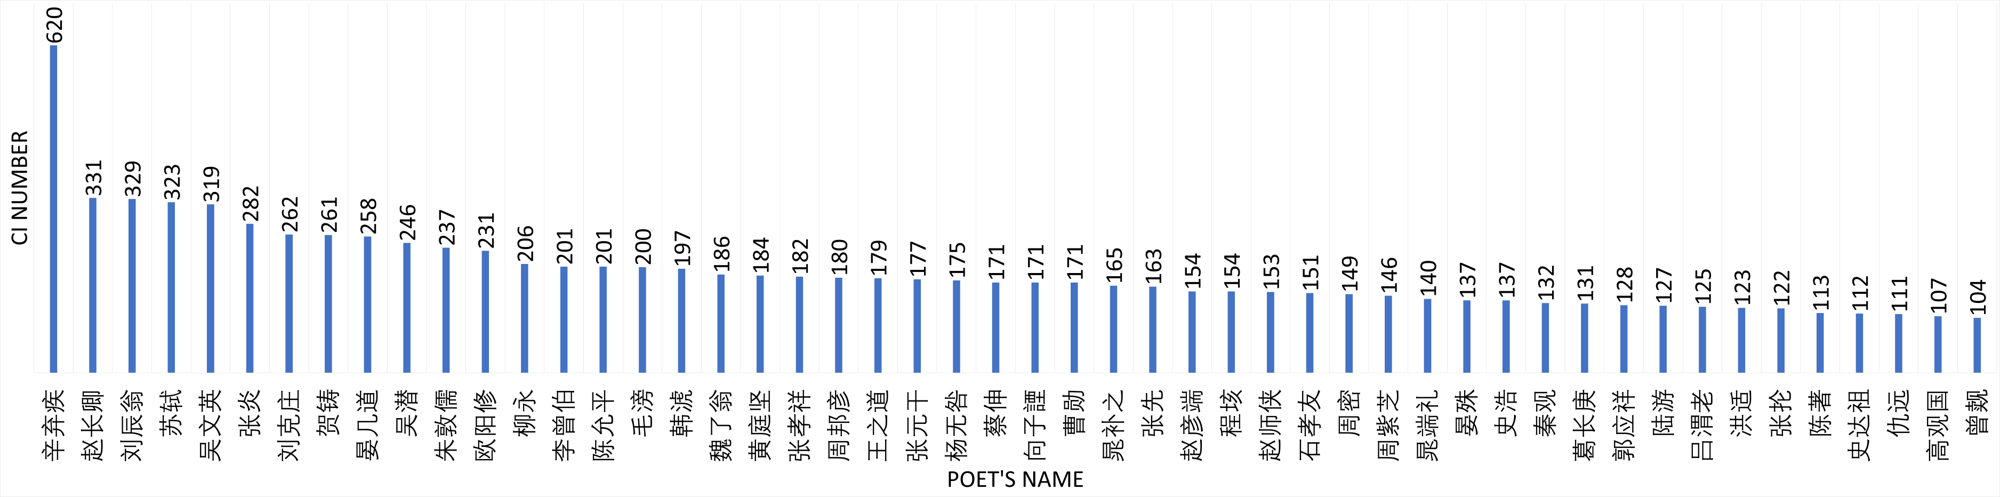
\includegraphics[width=0.9\linewidth]{poets.png}
	\caption{Poem Number Created by Top 50 Productive Poets}
	\label{fig:poet}
\end{figure}

\begin{figure}[htbp]
	\centering
	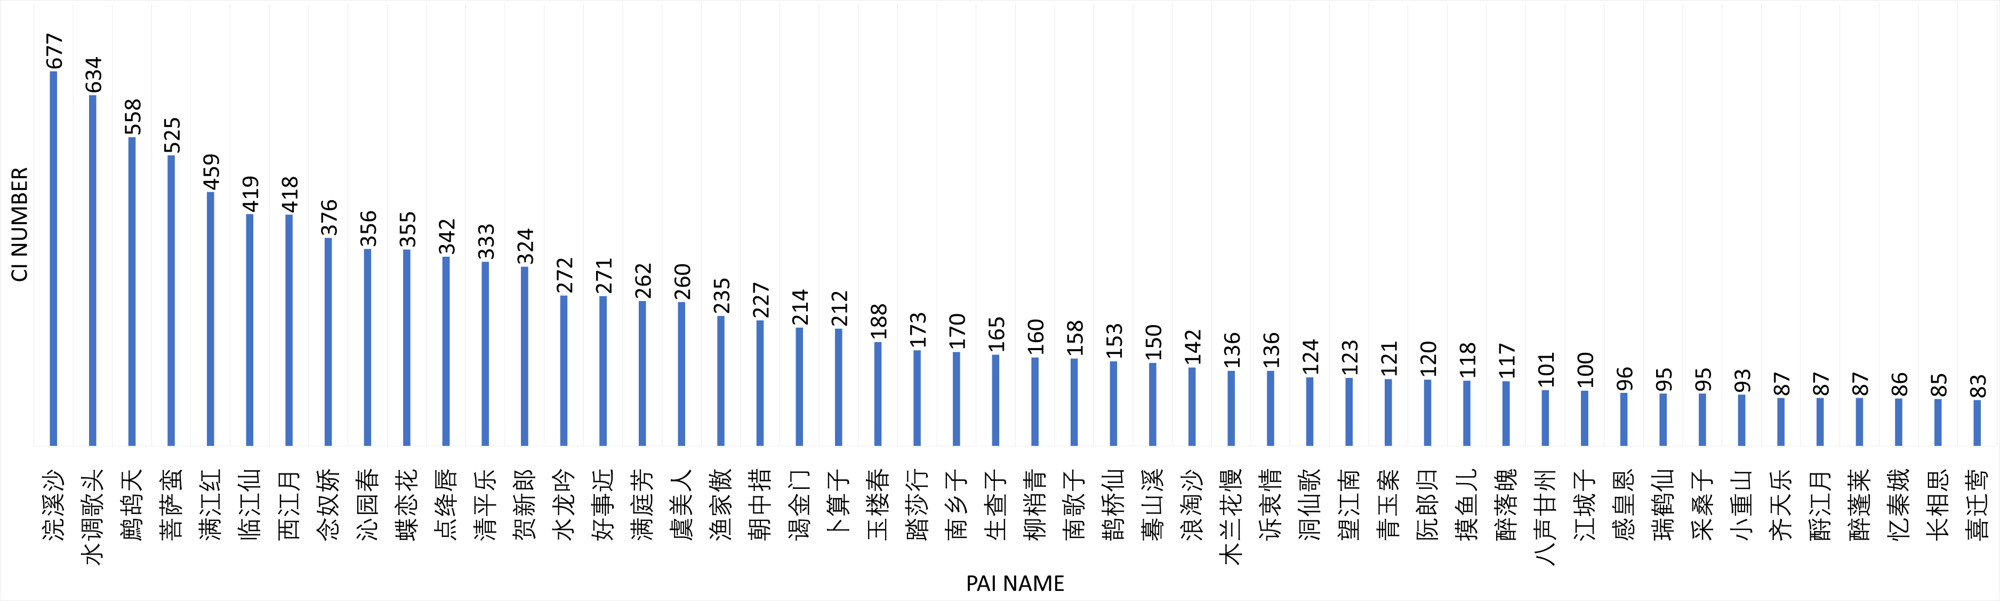
\includegraphics[width=0.9\linewidth]{Pai.png}
	\caption{Poem Number of Top 50 Popular Pai}
	\label{fig:pai}
\end{figure}
%

Word frequency analysis is to statistic and analyze the number of important words in the text, which is an important method of text mining. It is a traditional and useful content analysis method. The basic principle is to determine the overall style and theme of the entire article by the frequency of the words. By analyzing the word frequency in the poems, we have a general understanding of the style of poems and the process of writing those the poem, which can help us get more familiar with the grammar rules and themes of Ci. The most commonly used words can reveal common theme of Ci and the corresponding feelings. For example, we analyzed word frequency of season in our database. The result is shown in Figure \ref{fig:season}. We found that spring related words reached 2606, these words appeared in our dataset for 9210 times. Followed by autumn, there are 1167 words associated with autumn and appeared 3992 times. The unique scene in spring and autumn can trigger people's emotions, which might be the reason that so many poems are related with these two seasons.
\begin{figure}[htbp]
	\centering
	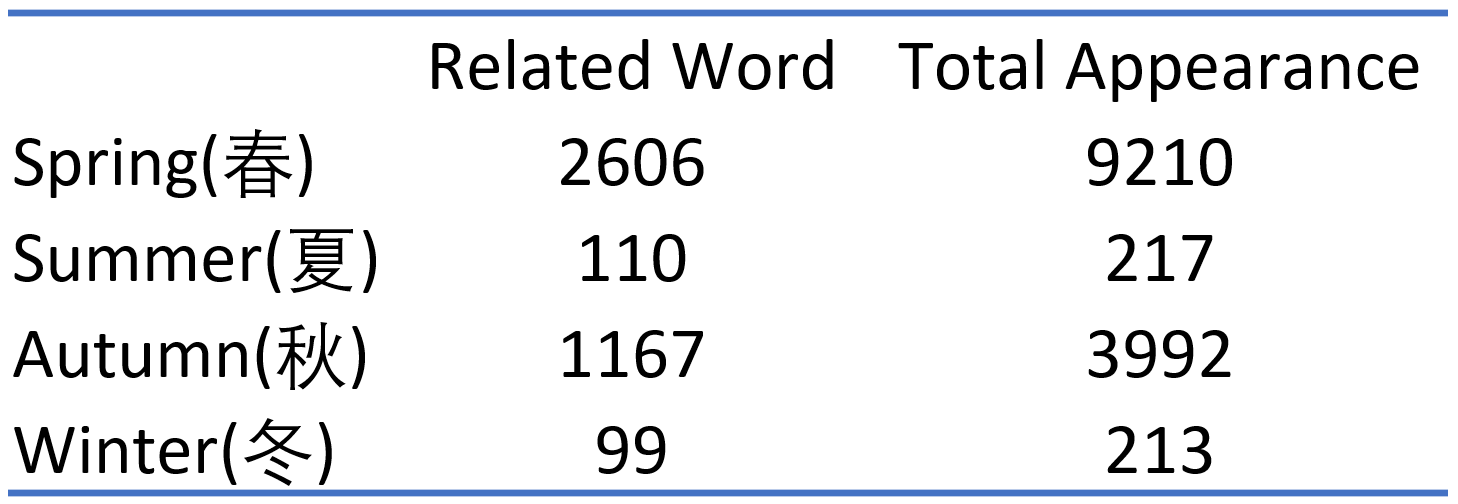
\includegraphics[width=0.8\linewidth]{season.png}
	\caption{Statistical Data of Season Related Word Frequency in Dataset}
	\label{fig:season}
\end{figure}
%
From most frequently used words, shown in Figure \ref{fig:wordcloud}, we found that the moon, east wind, mortal world, wine, dream, rain, flowers , sunset, old friends are the most commonly used images. Commonly used places, including Jiangnan, West Lake, Changan, Fairy Isle, Yangzhou. Commonly used verbs including laugh , come back, go back, lovesickness, look back, meet by chance. Commonly used emotions are hate, worry, hard, sigh, desolate, haggard. These words represent a very broad theme and style of Ci, including the description of leaving and missing, pride and enthusiasm, seasonal terms, chanting things, chanting nostalgia and so on.
%
\subsubsection{Implementation of Genetic Algorithm and Additional Information Collection}
Initially, we collect additional information about syntactic pattern of sentences with different length, format of tone pattern and rhythm and format of different Cipai from past research work on Song Ci.
%
The syntactic pattern for traditional Chinese poem are shown in Figure \ref{fig:syntactic}.
%
In this figure, sentence length means how many characters are in this sentence.
%
'*' in syntactic pattern represent a character and '/' used to split sentences into several parts.
%
Words in these sentence shell not cross the split.
%
Otherwise, this sentence may not be that easy to read and understand.
%
What we can see is that one several different syntactic patterns are allowed for the same sentence length, such as sentence with five characters, the sentence can either have two characters at the beginning then three characters or vice versa.
%
This actually gives traditional poems much freedom on expression.

\begin{figure}[htbp]
	\centering
	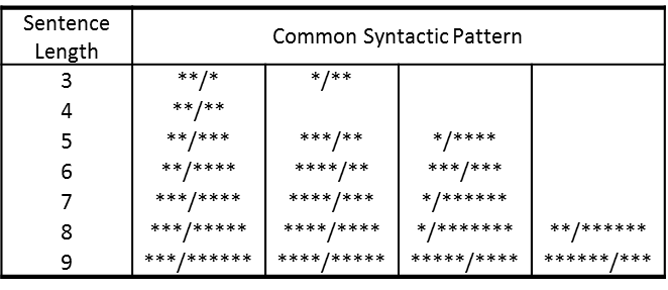
\includegraphics[width=0.9\linewidth]{syntactic.png}
	\caption{Syntactic Patterns for Sentences with Different Length.}
	\label{fig:syntactic}
\end{figure}

Then we defined several properties for characters and words in Song Ci.
%
Tone pattern which is called pingze in Chinese, we use 1 to represent Ping, 2 to represent Ze.
%
There are twenty four rhythm in Chinese, in traditional Chinese poem, usually the last characters of every sentence are required to be the same rhythm.
%
 We get pingze and rhythm information from existing datasets.
%
The correlation between words we use python package word2vec(https://code.google.com/archive/p/word2vec/) to quantify the relationship between words, which will be later used in generating Song Ci that is closely related with keywords.


We also extract format for different Cipai from existing dataset, which contains sentence number, length, tone pattern and the delimiter of each sentence.
%
For example, Huanxisha is a very popular Cipai in Song Ci.
%
The sentence format of Huanxisha is ['0201021', '0102211', '0102211', '0201122', '0102211', '0102211'].
%
In this format, there are 6 sentences, each sentence contains 7 characters.
%
0,1 and 2 represent the requirement of Pingze, 0 means both ping and ze will work in this position.
%
Each sentence will apply the syntactic pattern previous defined.


\begin{figure}[htbp]
	\centering
	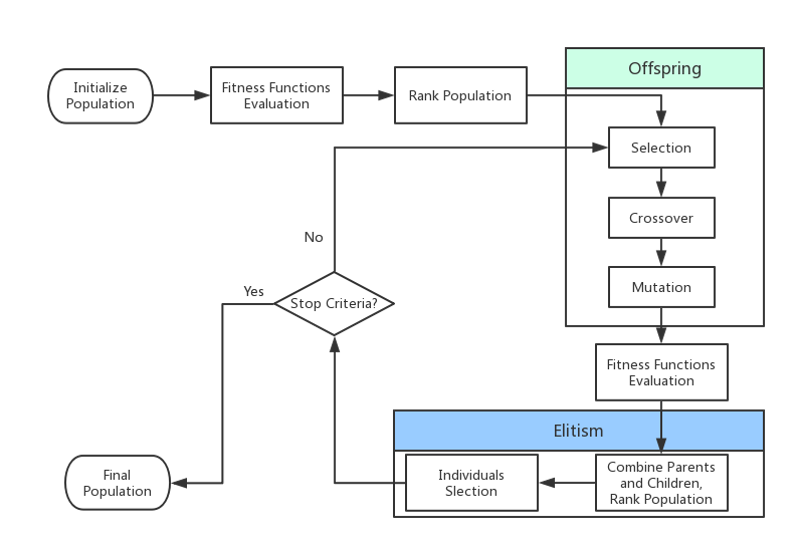
\includegraphics[width=0.9\linewidth]{GA.png}
	\caption{Process of Generating Song Ci by Genetic Algorithm}
	\label{fig:GA}
\end{figure}


Based on the rule of compose Song Ci, we found that Song Ci is a combination of words.
%
Thus, traditional method with pre-defined rules can easily generate Song Ci with correct format.
%
For genetic algorithm, we use a Cipai title and several keywords as input.
%
Based on the sentence format and tone requirement, words that are highly correlated with keywords are selected as candidate words for initial population.
%
Based on randomly chosen rhythm, pre-defined sentence form, syntactic patterns and tone patterns, program randomly put words that satisfied all the requirement to each position and generate the first generation of candidate poems.
%
The initial population is strictly follows the format and rules of Song Ci.


Then all candidate poems go through the fitness evaluation process.
%
Based on score of syntactic and semantic correctness, correlation with keywords, correlation between sentences and tone, rhythm pattern, a fitness value is generated for each candidate poem.
%
Best several individuals are selected as parents to generate offspring with mutation and crossover.
%
Mutation means characters within this poem will change randomly.
%
Crossover represents two poems randomly exchange part of their sentences and form two new poems.
%
All offspring and parents together forms the next generation and need to be evaluate on fitness value.
%
Then this iteration will continue until satisfactory fitness level has been reached or a maximum number of generations has been produced.


In the last, we'll manually choose best poem from the final generation.
%
The whole process is shown in Figure \ref{fig:GA}.
%
Final results are shown in following section.


\subsubsection{ Implementation of a Vector Space Model }
Vector space models (VSMs) represent words in a continuous vector space where semantically similar words are mapped to nearby points.
%
We implemented this model to find the semantic relations between each Chinese character, so that given a few of keyword characters, such as 'spring' and 'beauty', we can generate poetries with coherent meanings using characters which are close to these keywords in the vector space.
%
%We use a predictive method to implement this  model based on the TensorFlow programming package \cite{tensorflow}.
%
We give a visualized result in Figure \ref{fig:VSM}. The figure is embeded with 100 Chinese characters in a 2-D space, which are randomly chosen from the most frequent 500 Chinese characters in the Song Ci corpus. The 2-D space corresponds to the first two dimensions in the vector space. We can see that words such as `spring', `sunny', and `breeze' are very close in the 2-D space, which convey similar sentimental feelings to readers.



\begin{figure}[htbp]
	\centering
	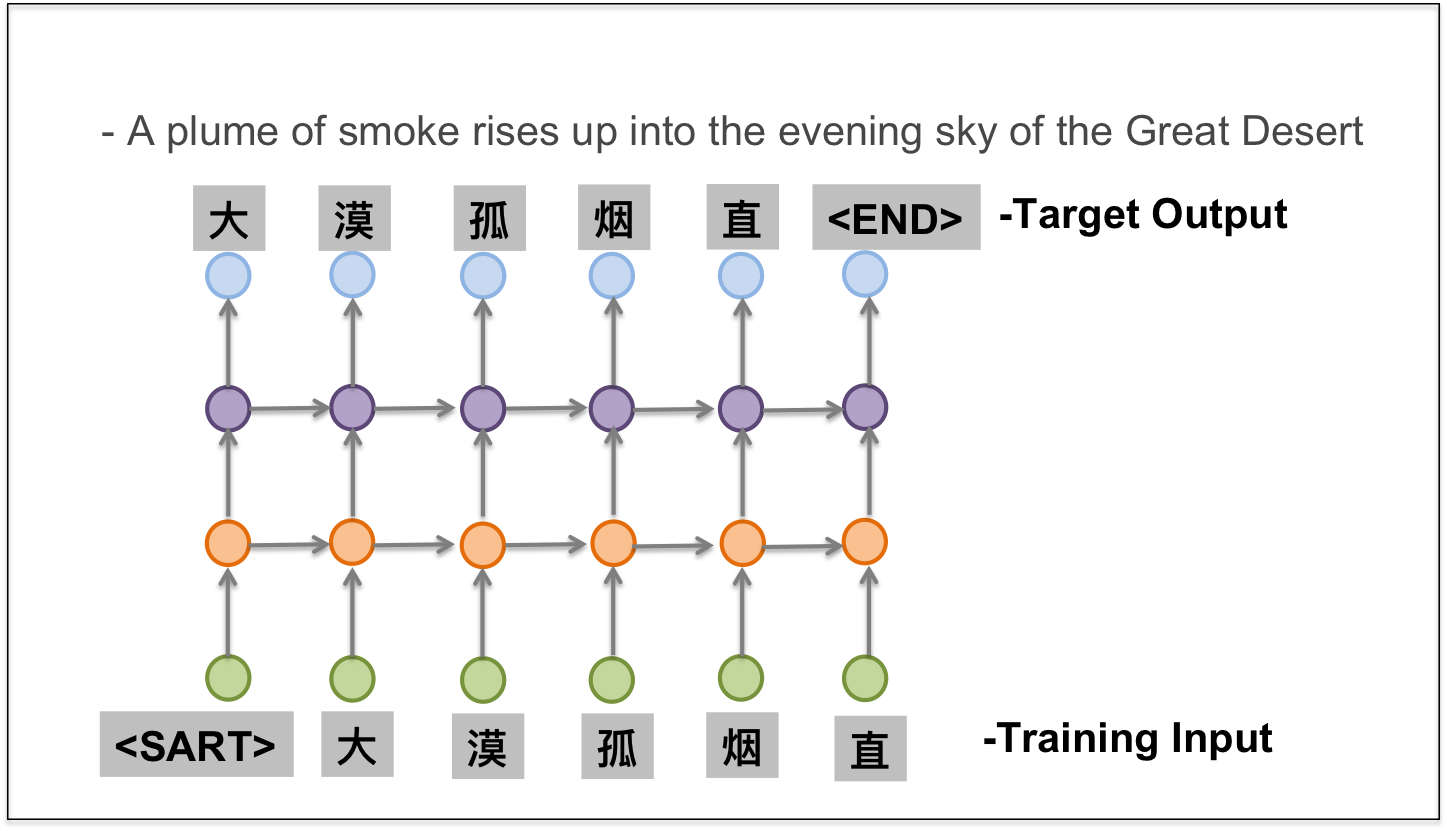
\includegraphics[width=0.9\linewidth]{RNN_model}
	\caption{Workflow of the RNN model}
	\label{fig:rnn_workflow}
\end{figure}

\begin{figure}[htbp]
	\centering
	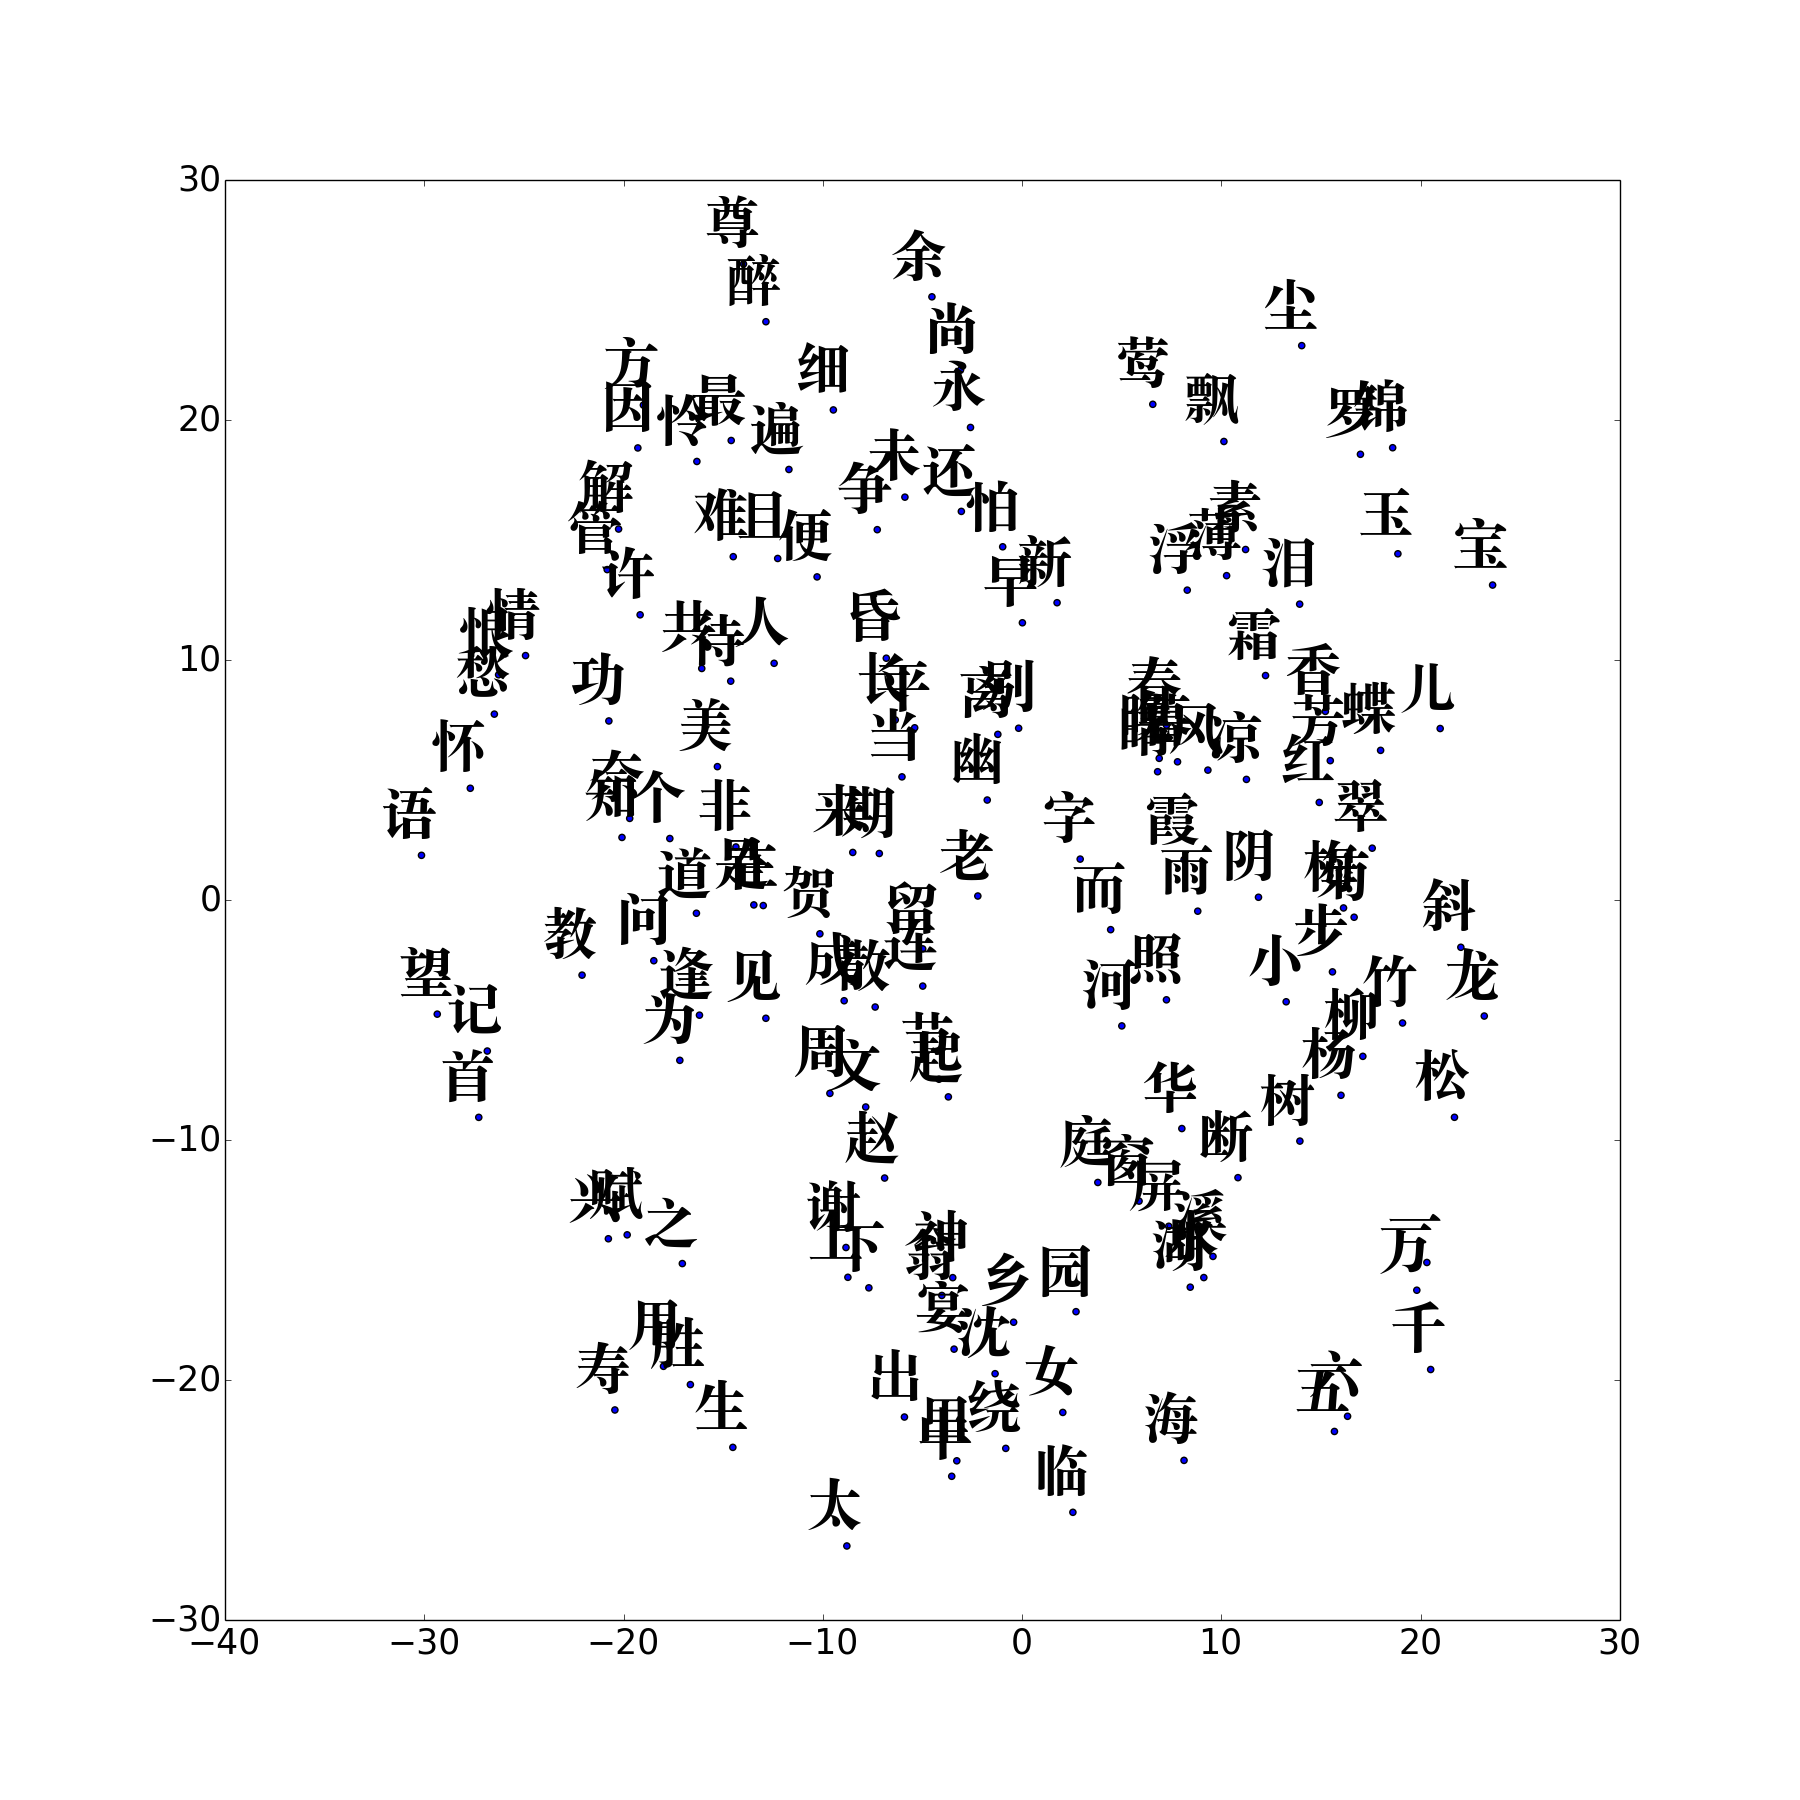
\includegraphics[width=0.9\linewidth]{tsne.png}
	\caption{Projections of most frequent characters to a 2-D space using the word embedding model}
	\label{fig:VSM}
\end{figure}



\subsubsection{Implementation of RNN Model} 
%
We used deep learning Python modules called \emph{TensorFlow} \cite{tensorflow} to implement our RNN model. 
%
We present a preliminary result in Figure \ref{fig:poetry}, which is a quatrain poem.
\begin{figure*}[htbp]
	\centering
	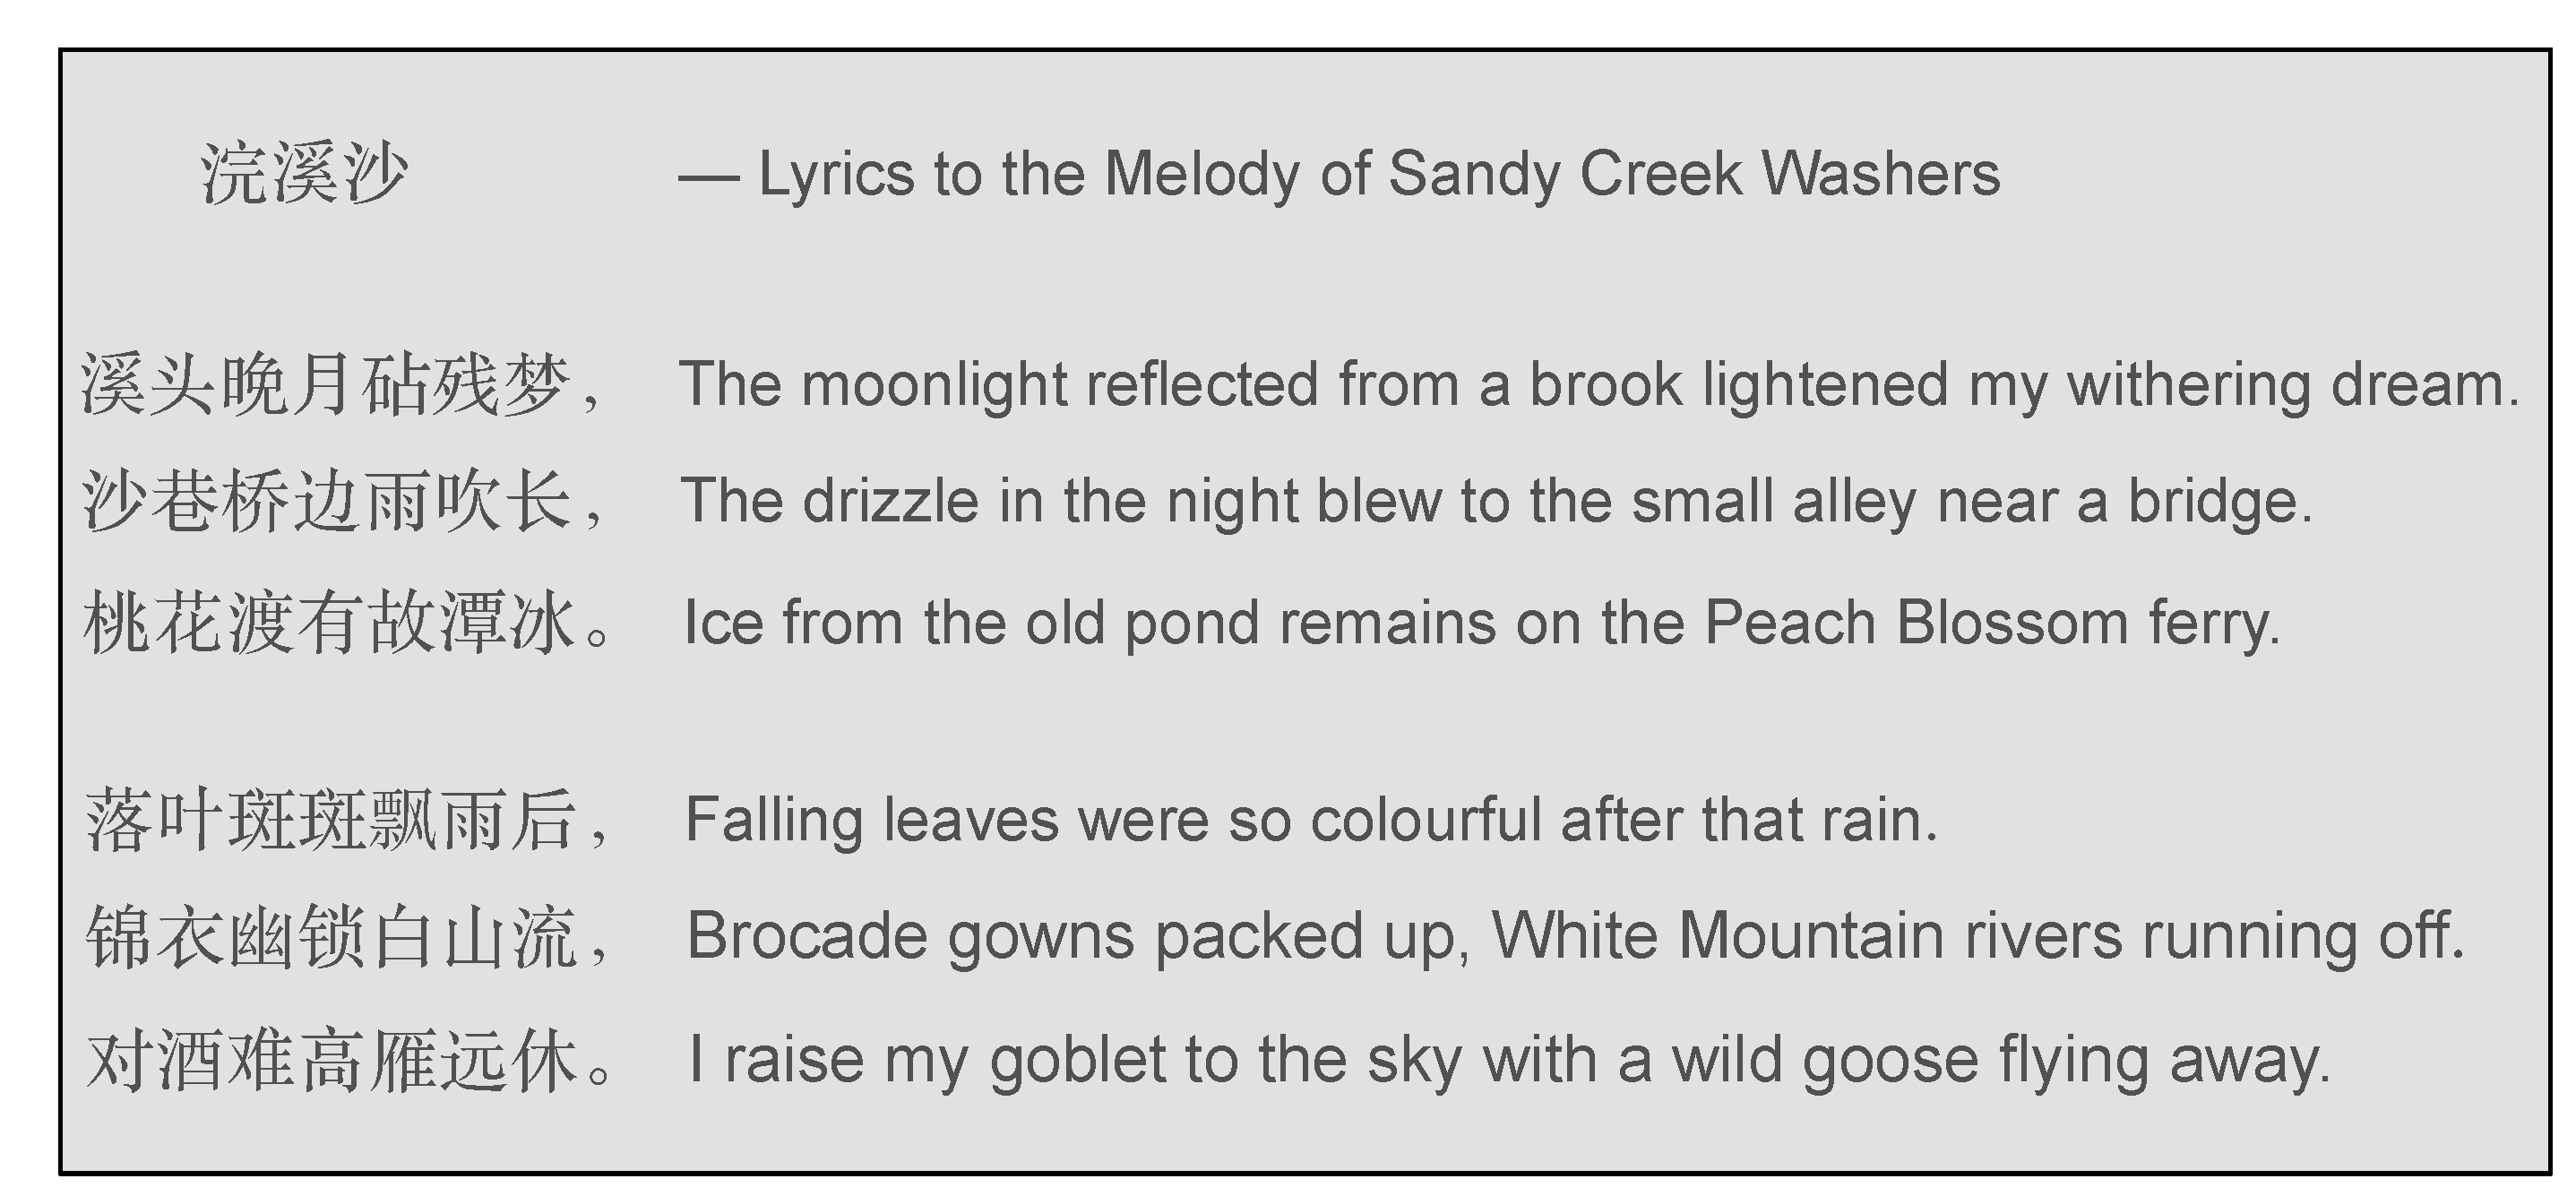
\includegraphics[width=0.8\linewidth]{poem_template}
	\caption{A Song Ci generated using LSTM}
	\label{fig:poetry}
\end{figure*}

\begin{figure*}[htbp]
	\centering
	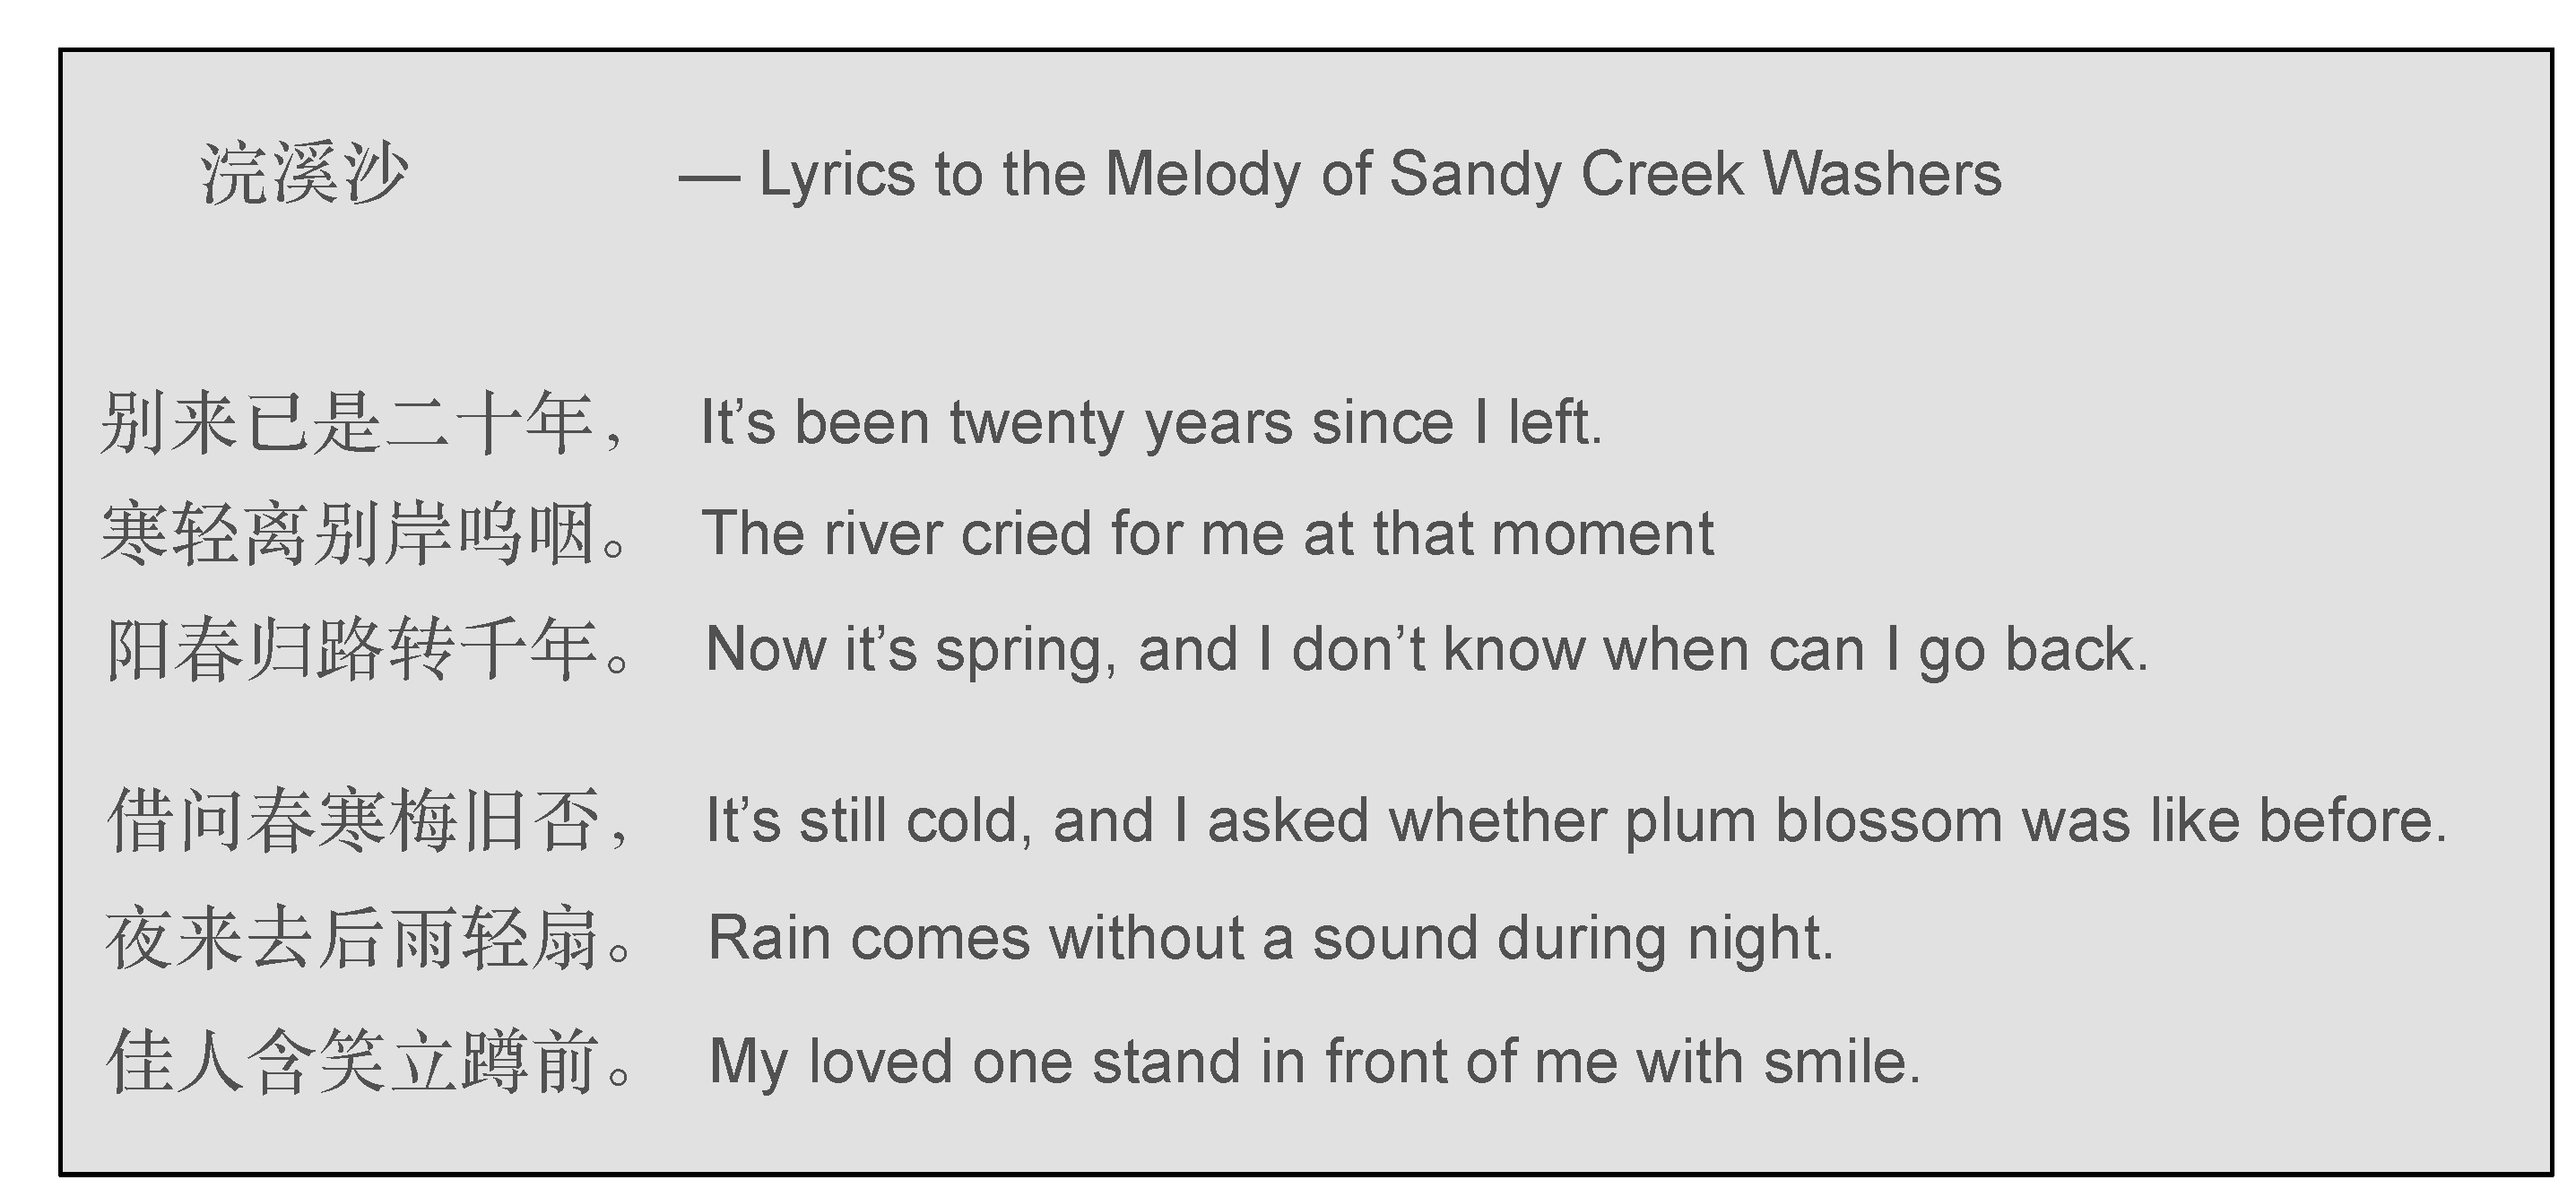
\includegraphics[width=0.8\linewidth]{poem_template2}
	\caption{A Song Ci generated using Genetic Algorithm }
	\label{fig:poetry}
\end{figure*}

\subsubsection{Implementation of SeqGAN Model} 

The SeqGAN model is implemented using TensorFlow \cite{tensorflow}. We first read all the data from text files, then convert all the Chinese character to integer vectors. Since Ci has different length, we also use the special placeholder to fill the space after the end of the text. The sequence length is adjusted based on task. For general Ci generation, we use 128 as sequence length. For Huanxisha generation, we use 48 as sequence length. We use an adaptive learning optimization algorithm called Adam \cite{kingma2014adam} to optimize our CNNs with initial learning rate $ =  0.01 $.

For the generator, we use LSTM cell \cite{hochreiter1997lstm} as the unit of hidden layers of recurrence neural networks. Right now, our implementation has 64 units in the hidden layers of RNNs.

The discriminator is a convolutional neural network for 2 classes classification. The input matrix is from the embedding of discrete tokens. Convolutional kernel applied to the input matrix to extract features. In our implementation, all convolution operation use $ [1, 1, 1, 1]  $ as its strides and valid padding. In the real implementation, a series of the diffrent number of the convolutional kernel with different window size is applied to extract different features. The model also adopt highway structure \cite{srivastava2015highway} and dropout (dropout rate $ = 0.25 $)\cite{hinton2012dropout} to further improve the performance. The loss function of CNNs is cross entropy loss function with l2 norm regularization term. In the experiment, the coefficient of l2 norm $ \lambda =  0.2 $. We use an adaptive learning optimization algorithm called Adam \cite{kingma2014adam} to optimize our CNNs with initial learning rate $ =  1e^{-4} $. We still use Adam optimizer with $ 1e^{-4} $ as its learning rate.

To train the SeqGAN model, we use the computational node provided by High-Performance Computing Center from Michigan State University. Most training job running use a single Nvidia Tesla K80 GPU in the  intel16-k80 clusters. For Huanxisha generation, a 12-hour job generates 79000 poems.

% !TEX root = /Users/zhuzhuangdi/Desktop/MSUCourses/MachineLearning847/17spr_wang_zhu_du/Final/final_report.tex
\section{Conclusion and Future Work} 

In this project, we propose and implement three different approaches to generate Chinese Song Ci automatically: a traditional Genetic Algorithm Model, a Recurrent Neural Network model, and a Generative Adversarial Network model, respectively.
%
For traditional approach, its advantage is that the output will always follow the structure or rhyme rules of Song Ci by evaluating each candidate agains an evaluation function,  and only the candidate with a satisfying evaluation value will be chosen as the output.
%
For the two deep learning approaches using neural networks, its advantage is that no pre-definend constraints are need for the model, as  the sophisticated rules for each genre of Song Ci can be learned automatically by a large set of training data.

The human evaluation shows that all of the three approaches succeed in generating Song Ci with the correct structure and gramma rules. For GA model and RNN model, not only can they generate Song Ci with the same rhymes, they can also generate Song Ci with consistent semantic meanings which receives high scores by human evaluation. 

To further improve the qualities of generation, we can adopt the knowledge based method that can incorporate extra sources of knowledges. Previews work \cite{wang2016baidu} showed that by using extract knowledges from encyclopedia, the RNNs model can write the poem in topic which cannot find in the ancient Chinese poems. 

Also, a systematic evaluation is necessary to rate each model. Popular automatic evaluation method, like BLEU, cannot provide a comprehensive metric as human evaluation\cite{iu2016evaluate}. For this reason, we may need to organize human evaluation to evaluate all the results generated by our models.

Finally, RNNs has various structures and we may benefit from advanced RNN models. For example, attention-based RNN and Lookback RNN \cite{lookbackRNN} already prove it can efficiently generate musics. These models should further improve the results.


Our future work would be applying our models to other forms of text generation task, such as generating Yuan Qu, or generating poems in other languages.


\bibliographystyle{abbrv}
\bibliography{final_report}
\end{document}
